% AUTO-GENERATED FILE. DO NOT EDIT DIRECTLY.
% Source: docs/report/chapter-3-system-design-and-methodology.md
% Regenerate with: python3 scripts/migrate_markdown_to_latex.py

\hypertarget{chap:ch3}{%
\chapter{System Design and Methodology}\label{chap:ch3}}

Chapter~\ref{chap:ch2} identified several unresolved problems in long-term conversational memory. Storage and retrieval are often changed together, which makes their effects difficult to separate. Curated memory can improve organisation but may also omit or alter information. Selective retrieval can reduce context length, but it can fail to surface required evidence. Complete context avoids explicit retrieval omission, yet it may introduce noise and long-context utilisation problems. A final answer score alone does not reveal which stage caused an error.

This chapter translates these general problems into a concrete system design. The study separates memory representation, evidence retrieval, evidence packaging, and answer generation. It then derives a set of conditions that supports controlled component comparisons, complete-system comparisons, dual-source fusion, and comparison with a no-retrieval Full Context path.

The chapter explains why the system has this structure and how its components operate. Method-defining constants are introduced where their mechanisms are specified. Chapter~\ref{chap:ch4} consolidates the experimental settings and defines the frozen question set, backbone models, remaining run controls, execution protocol, evaluation metrics, and statistical analyses. Chapter~\ref{chap:ch5} presents and interprets the results. The purpose of this chapter is therefore to define the system and justify the condition structure, rather than to determine which condition performs best.

\hypertarget{sec:ch3-1}{%
\section{From Research Gaps to Methodological Requirements}\label{sec:ch3-1}}

\hypertarget{sec:ch3-1-1}{%
\subsection{Separating Storage, Retrieval, and Answering}\label{sec:ch3-1-1}}

A long-term memory system should not be treated as one indivisible component. Its end-to-end process can be divided into four stages:

\[
\begin{aligned}
\text{Conversation history}
&\rightarrow \text{Memory representation} \\
&\rightarrow \text{Retrieval and evidence selection} \\
&\rightarrow \text{Answer generation}.
\end{aligned}
\]

Each stage can produce a different type of failure. The required information may not be retained when the memory is constructed. It may be present in the memory but remain unretrieved. Relevant material may appear in search results but not be selected for the final evidence input. Evidence may also be removed by a fixed budget. Finally, complete evidence may reach the Answerer but still be interpreted incorrectly.

These cases require different remedies. A write omission requires a better memory-construction process. A retrieval omission requires a better search strategy. Evidence loss may require a different packaging or budget policy. A utilisation error instead concerns the Answerer's ability to interpret the available evidence. One end-to-end answer score cannot distinguish among these mechanisms.

Building on the retrieval-to-generation separation in \cite{yuan2026retrievalutilization}, the system therefore makes storage, retrieval, evidence packaging, and answering explicit. This four-stage distinction is a project-specific extension: \cite{yuan2026retrievalutilization} groups missing stored detail and missed retrieval under one retrieval-stage category. Each retriever produces an inspectable retrieval trace and a standardised EvidenceBundle. The Answerer operates only after retrieval has ended. This separation supports later analysis of where relevant information was preserved, found, retained, and used.

\hypertarget{sec:ch3-1-2}{%
\subsection{Requirement 1: Isolating Storage Organisation}\label{sec:ch3-1-2}}

Prior studies compare flat or raw archives with structured, curated, or summarised memory variants \cite{zhou2026filesystem,yuan2026retrievalutilization}. Such a comparison can change both content and organisation. Any observed difference may result from rewritten text, removed detail, new semantic labels, or a different path structure.

The present study introduces two raw memory representations to isolate directory organisation. S1 stores the original sessions in one flat directory. S2 places the same complete session files into topic directories. The intended content relationship is:

\[
\operatorname{content}(S1)=\operatorname{content}(S2),
\]

while their path structures differ:

\[
\operatorname{paths}(S1)\neq\operatorname{paths}(S2).
\]

S2 does not summarise, split, merge, or rewrite a session. It only adds a directory hierarchy. This creates a controlled way to ask whether navigational structure helps memory access when the underlying dialogue remains unchanged.

The comparison does not measure semantic compression or fact extraction. It is restricted to the incremental effect of directory organisation and the way a retriever responds to that organisation.

\hypertarget{sec:ch3-1-3}{%
\subsection{Requirement 2: Comparing Retrieval Strategies on the Same Memory}\label{sec:ch3-1-3}}

A storage representation cannot be assessed independently if every store is paired with a different retriever. The study therefore applies two retrieval families to both raw stores. On S1, R1 defines E1 and R2 defines E2. On S2, the corresponding conditions are E3 and E4. These four conditions form the controlled raw-memory core.

Holding the memory representation constant supports two retrieval comparisons. E2 versus E1 compares R2 with R1 on flat raw sessions. E4 versus E3 compares the same retrieval families on foldered raw sessions. Holding the retrieval family constant supports two storage comparisons. E3 versus E1 examines how directory organisation affects R1, while E4 versus E2 examines whether the same organisation also affects R2.

The four conditions also support an interaction question: does directory organisation help one retrieval family more than the other? R1 can inspect and navigate paths directly. R2 instead begins from lexical ranking over raw conversation units. The R2 index excludes directory names, so the same query and date filter produce the same first-stage ranking over S1 and S2. However, result provenance can expose an S2 path to the Retrieval Agent. That path may influence a later query. Directory structure can therefore affect adaptive retrieval even when it is excluded from lexical scoring.

This is a controlled partial-factorial core rather than a claim that all retrieval interfaces are identical. Each retrieval family requires representation-appropriate observations and instructions. Chapter~\ref{chap:ch4} defines the paired contrasts and controls used when interpreting them.

\hypertarget{sec:ch3-1-4}{%
\subsection{Requirement 3: Evaluating Curated Memory as a Complete System}\label{sec:ch3-1-4}}

S3 differs fundamentally from S1 and S2. It is an agent-curated memory rather than a relocated copy of the raw dialogue. Its construction process can rewrite statements, combine evidence from several sessions, group facts by entity and topic, reconcile later updates, and remove repetition. It can also omit qualifiers, preserve an outdated state, or join facts incorrectly.

S3 must therefore be evaluated as a complete representation rather than as a third directory layout. The study provides two ways to access the same frozen S3 store:

\begin{itemize}
\tightlist
\item
  E5 combines S3 with R1, the general filesystem retriever.
\item
  E6 combines S3 with R3, a retrieval adapter designed for factual units and topic groups.
\end{itemize}

This pair addresses two questions. First, can a general filesystem Retrieval Agent use a curated store effectively? Second, does a retriever adapted to the internal structure of curated memory access the same store differently?

The conditions do not form an exhaustive \(3\times3\) storage--retrieval matrix. R2 and R3 are not two independent generic retrievers. R2 operates over exchanges grouped by raw sessions. R3 adapts the same broad iterative retrieval principle to curated facts grouped by topic sections. R3 is therefore representation-specific. By contrast, R1 can browse S1, S2, and S3 through a common filesystem interface.

The condition set includes theoretically meaningful and operationally valid pairings rather than every nominal combination. Comparisons involving S3 must also remain system-level comparisons. Since S3 changes content, granularity, organisation, and provenance presentation together, a difference between S3 and a raw store cannot be attributed to one isolated storage feature.

\hypertarget{sec:ch3-1-5}{%
\subsection{Requirement 4: Testing Raw--Curated Complementarity}\label{sec:ch3-1-5}}

Raw dialogue and curated memory provide different forms of evidence. Raw dialogue retains exact wording, local context, temporal order, and complete source history. Its information may nevertheless be dispersed across many sessions and surrounded by irrelevant material. Curated memory can consolidate related facts and organise them by entity and topic. However, curation may omit detail, alter wording, or combine inconsistent states.

The two sources may therefore be complementary. Raw evidence may repair a write omission or distortion in curated memory. Curated evidence may connect facts that remain separated in raw sessions. Conversely, combining the sources may introduce duplication, conflicting descriptions, or additional distraction.

E7 tests this relationship by combining the EvidenceBundles already produced by E2 and E6. E2 represents raw dialogue accessed through the raw-chat retrieval path. E6 represents curated memory accessed through its adapted retrieval path. This pairing is fixed by the system design and is not selected after observing performance.

E7 does not formulate a new query or execute a third retriever. It performs deterministic post-retrieval fusion and then invokes the shared Answerer once. The condition therefore examines whether already retrieved raw and curated evidence are complementary or interfering.

\hypertarget{sec:ch3-1-6}{%
\subsection{Requirement 5: Distinguishing Retrieval Failure from Long-Context Failure}\label{sec:ch3-1-6}}

A failed selective-retrieval answer does not show whether the Answerer lacked the required information or failed to use it. To support this distinction, the study adds a Full Context diagnostic path. Full Context sends the complete ordered raw conversation directly to the Answerer without an external retrieval stage.

This path supports several diagnostic questions. If Full Context repairs an error made by selective retrieval, the selective path may have omitted necessary evidence. If selective retrieval succeeds while Full Context fails, evidence selection may have reduced distracting material. If both paths receive the required material but still fail, the result indicates a downstream utilisation or reasoning problem \cite{yuan2026retrievalutilization}. Subsequent analysis can then test question-specific mechanisms such as temporal ordering, entity resolution, multi-source composition, and long-context position effects \cite{liu2024lost}.

Full Context is not a fourth memory representation, a fourth retriever, or an eighth selective condition. It is also not an oracle. Complete source visibility does not guarantee correct use. It is a separate no-retrieval path used to examine the consequences of removing explicit evidence selection.

\hypertarget{sec:ch3-1-7}{%
\subsection{Requirement 6: Controlling the Answering Stage}\label{sec:ch3-1-7}}

A comparison of memory access becomes difficult to interpret if every retriever uses a different evidence format or answering prompt. The study therefore requires all selective conditions to follow the same downstream structure:

\[
\begin{aligned}
\text{Condition-specific retrieval}
&\rightarrow \text{Common EvidenceBundle} \\
&\rightarrow \text{Shared Answerer} \\
&\rightarrow \text{Common output schema}.
\end{aligned}
\]

The Answerer receives the question, an ordered EvidenceBundle, and shared answering instructions. It does not receive the condition identifier, retriever name, retrieval score, retrieval trace, reference answer, gold evidence, or evaluation label. It also has no retrieval tools. Its task begins only after the evidence input has been finalised.

The same component graph and interface definitions are used when the experiment is instantiated with different backbone models. Within each backbone pipeline, the selective conditions use the same Answerer protocol. Chapter~\ref{chap:ch4} describes the backbone deployments and identifies which factors remain fixed across them.

\hypertarget{sec:ch3-1-8}{%
\subsection{Derivation of the Final Condition Set}\label{sec:ch3-1-8}}

The preceding requirements lead to four related parts of the study. E1--E4 form the controlled raw-memory core. E5--E6 extend the design to agent-curated memory. E7 tests dual-source evidence fusion. Full Context removes explicit retrieval as a diagnostic comparison.

\setcounter{table}{0}
\begingroup
\renewcommand{\theHtable}{\thechapter.\arabic{table}.block1}
\fontsize{5.0pt}{5.45pt}\selectfont
\setlength{\tabcolsep}{0.7pt}
\renewcommand{\arraystretch}{0.82}
\hfuzz=\maxdimen
\vfuzz=\maxdimen
\begin{longtable}[]{@{}
  >{\raggedright\arraybackslash}p{(.96\columnwidth - 4\tabcolsep) * \real{0.33}}
  >{\raggedright\arraybackslash}p{(.96\columnwidth - 4\tabcolsep) * \real{0.33}}
  >{\raggedright\arraybackslash}p{(.96\columnwidth - 4\tabcolsep) * \real{0.33}}@{}}
\caption[Derivation of the system conditions from the research problems.]{Derivation of the system conditions from the research problems.}\label{tab:ch3-1}\\
\toprule
Research problem & Design response & Relevant conditions or path \\
\midrule
\endfirsthead
\multicolumn{3}{r}{\small\itshape Continued from the previous page}\\
\toprule
Research problem & Design response & Relevant conditions or path \\
\midrule
\endhead
Storage organisation is confounded with content transformation & Compare flat and foldered stores with identical raw session contents & E1/E3 and E2/E4 \\
Retrieval effects are confounded with storage effects & Apply R1 and R2 to the same raw stores & E1--E4 \\
Curated memory changes both content and structure & Evaluate one S3 store through general and adapted retrieval & E5 and E6 \\
Raw and curated evidence may be complementary & Fuse the existing E2 and E6 EvidenceBundles & E7 \\
Retrieval omission is difficult to separate from utilisation failure & Remove selective retrieval and expose the complete raw history & Full Context \\
Answer generation may confound memory comparisons & Use a shared EvidenceBundle and Answerer protocol & E1--E7 \\
\bottomrule
\end{longtable}
\endgroup

The resulting design is theory-driven rather than an exhaustive Cartesian product. Each condition has a defined role in isolating raw-store organisation, comparing retrieval behaviour, examining curated-memory access, testing evidence fusion, or removing explicit retrieval.

\hypertarget{sec:ch3-2}{%
\section{Task Formalisation}\label{sec:ch3-2}}

\hypertarget{sec:ch3-2-1}{%
\subsection{Conversation, Session, and Source Turn}\label{sec:ch3-2-1}}

Let a conversation be an ordered sequence of sessions:

\[
\mathcal{C}=(\sigma_1,\sigma_2,\ldots,\sigma_M).
\]

Each session \(\sigma_i\) is an ordered sequence of source turns:

\[
\sigma_i=(u_{i,1},u_{i,2},\ldots,u_{i,n_i}).
\]

LoCoMo supplies ordered sessions, speaker contributions, session dates, dialogue text, optional image captions, and answer-source turn identifiers \cite{maharana2024locomo}. In this study, a \textbf{source turn} is one such speaker contribution. The local canonicaliser preserves the source fields and adds a stable project locator and content identity.

The report uses \emph{source turn} rather than the unqualified term \emph{turn}. This avoids confusion with the larger exchange units used by R2 and with the reasoning rounds used by R1.

\hypertarget{sec:ch3-2-2}{%
\subsection{Question and Evaluation-Only Information}\label{sec:ch3-2-2}}

Let \(q\) denote the question presented to the retrieval and answering pipeline. During online execution, the system may access \(q\) and the permitted memory representation. It cannot access the reference answer or the benchmark's annotated evidence.

Let \(a^*\) denote the reference answer. Let \(G_q\) denote the set of annotated gold source identifiers when such evidence is available. The question category and evaluation scores are also evaluation-only information. These fields are introduced only after the candidate answer has been generated.

This boundary applies to every online component. The memory-construction process, Retrieval Agent, deterministic retrieval backend, fusion procedure, and Answerer cannot use \(a^*\), \(G_q\), or any evaluation label.

\hypertarget{sec:ch3-2-3}{%
\subsection{Memory Representation}\label{sec:ch3-2-3}}

A memory representation is a transformation of the same canonical conversation:

\[
\mathcal{M}_s=T_s(\mathcal{C}),
\qquad s\in\{1,2,3\}.
\]

Here, \(\mathcal{M}_1\), \(\mathcal{M}_2\), and \(\mathcal{M}_3\) correspond to S1, S2, and S3. A representation includes both its text and its access-relevant structure. This structure may include filenames, directory paths, headings, topic groups, session boundaries, and source locators.

The transformation \(T_s\) does not imply that every store rewrites the source. S1 and S2 serialise the raw sessions without rewriting their contents. S3 instead produces curated factual memory through an agent-managed construction process.

\hypertarget{sec:ch3-2-4}{%
\subsection{Retrieval Trace and Evidence Selection}\label{sec:ch3-2-4}}

For a compatible memory representation and retrieval system, retrieval is defined as:

\[
\mathcal{R}_r(q,\mathcal{M}_s)
\rightarrow
(\tau_{s,r,q},\mathcal{B}_{s,r,q}),
\]

where \(\mathcal{R}_r\) is the retrieval system, \(\tau_{s,r,q}\) is the retrieval trace, and \(\mathcal{B}_{s,r,q}\) is the resulting EvidenceBundle.

A retrieval trace is an ordered sequence of observations and actions:

\[
\tau=((o_1,a_1),(o_2,a_2),\ldots,(o_L,a_L)).
\]

Depending on the retriever, a trace may include directory observations, file reads, search expressions, generated lexical queries, ranked results, evidence-selection decisions, seen-state, and stopping decisions. R1 measures interaction through provider rounds, whereas R2 and R3 use bounded controller actions. These units are not assumed to be equivalent and are defined separately in Section~\ref{sec:ch3-6}.

\hypertarget{sec:ch3-2-5}{%
\subsection{EvidenceBundle}\label{sec:ch3-2-5}}

An EvidenceBundle is an ordered sequence of validated EvidenceItems:

\[
\mathcal{B}=(e_1,e_2,\ldots,e_K).
\]

Each item contains exact evidence text and the metadata required to identify its origin. Conceptually, this includes an evidence identifier, source kind, file path or structural group, source locators, canonical source identifiers, dates, speakers where applicable, content identity, and selection order.

The model does not provide arbitrary text as formal evidence. It selects material that has appeared in a valid observation. The host then re-reads the declared source and resolves the final text and provenance. This distinction separates model-directed selection from evidence authenticity.

\hypertarget{sec:ch3-2-6}{%
\subsection{Answer Generation}\label{sec:ch3-2-6}}

Let \(A_\theta\) denote the Answerer instantiated with backbone model parameters \(\theta\). For a selective-retrieval condition, answer generation is:

\[
\hat{a}=A_\theta(q,\mathcal{B}),
\]

where \(\hat{a}\) is the candidate answer.

The Answerer receives only the question, the final ordered evidence, and the shared answering instructions. It does not inspect the retrieval trace or access the memory store directly.

For Full Context, the evidence-access path changes:

\[
\hat{a}_{FC}=A_\theta(q,\mathcal{C}).
\]

Conceptually, the complete ordered raw conversation replaces a selectively constructed EvidenceBundle. In the shared Answerer interface, the complete session bodies are still wrapped as non-selective EvidenceItems so that provenance and citation validation remain available. The Answerer remains responsible for producing the candidate response, but no external retriever selects the preceding context.

\hypertarget{sec:ch3-2-7}{%
\subsection{RunRecord and Offline Evaluation Record}\label{sec:ch3-2-7}}

An online RunRecord can be represented as:

\[
r=(q,c,\tau,\mathcal{B},\hat{a},\rho),
\]

where \(c\) identifies the system condition and \(\rho\) contains operational metadata such as model-call and token measurements. For Full Context, the retrieval trace and selective EvidenceBundle are absent. The record instead contains the non-selective full-context bundle and identifies its complete source input.

An offline evaluation record is created after answer generation:

\[
z=(r,a^*,G_q,\mathbf{s}),
\]

where \(\mathbf{s}\) is the vector of answer, evidence, and process measures defined in Chapter~\ref{chap:ch4}. Separating \(r\) from \(z\) makes the evaluation boundary explicit. Gold information is attached to an existing answer record rather than supplied to the online pipeline.

\setcounter{table}{1}
\begingroup
\renewcommand{\theHtable}{\thechapter.\arabic{table}.block2}
\fontsize{5.0pt}{5.45pt}\selectfont
\setlength{\tabcolsep}{0.7pt}
\renewcommand{\arraystretch}{0.82}
\hfuzz=\maxdimen
\vfuzz=\maxdimen
\begin{longtable}[]{@{}ll@{}}
\caption[Principal notation used in the system definition.]{Principal notation used in the system definition.}\label{tab:ch3-2}\\
\toprule
Symbol & Meaning \\
\midrule
\endfirsthead
\multicolumn{2}{r}{\small\itshape Continued from the previous page}\\
\toprule
Symbol & Meaning \\
\midrule
\endhead
\(\mathcal{C}\) & Complete ordered conversation \\
\(\sigma_i\) & Session \(i\) \\
\(u_{i,j}\) & Source turn \(j\) in session \(i\) \\
\(q\) & Online question \\
\(a^*\) & Reference answer used only for evaluation \\
\(G_q\) & Annotated gold source set, where applicable \\
\(T_s\) & Transformation that constructs memory representation \(s\) \\
\(\mathcal{M}_s\) & Memory representation S1, S2, or S3 \\
\(\mathcal{R}_r\) & Retrieval system R1, R2, or R3 \\
\(\tau\) & Retrieval trace \\
\(e_k\) & One validated EvidenceItem \\
\(\mathcal{B}\) & Ordered EvidenceBundle \\
\(A_\theta\) & Answerer using backbone model parameters \(\theta\) \\
\(\hat{a}\) & Candidate answer \\
\(r\) & Online RunRecord \\
\(z\) & Offline evaluation record \\
\(\mathbf{s}\) & Evaluation metric vector \\
\bottomrule
\end{longtable}
\endgroup

\hypertarget{sec:ch3-3}{%
\section{Overall System Architecture}\label{sec:ch3-3}}

\hypertarget{sec:ch3-3-1}{%
\subsection{Layered System Structure}\label{sec:ch3-3-1}}

The system contains six logical layers. The first layer is the canonical source conversation. It preserves the original session order, source turns, dates, speakers, dialogue identifiers, and available captions.

The second layer performs normalisation and establishes provenance. It converts the source into canonical records, raw session files, exchange units, and a common source map. These artefacts provide the shared foundation for all later paths.

The third layer contains the three memory representations. S1 preserves raw sessions in a flat directory. S2 preserves the same session contents under a topic hierarchy. S3 stores agent-curated facts organised by entity and topic.

The fourth layer performs evidence access. R1 navigates the filesystem directly. R2 performs iterative lexical retrieval over raw exchanges and sessions. R3 adapts this iterative approach to curated facts and topic groups. The Full Context path bypasses this layer.

The fifth layer standardises the retrieved information. All selective paths produce the same conceptual EvidenceBundle before answer generation. E7 operates at this layer by fusing the completed bundles from E2 and E6.

The sixth layer contains the shared Answerer and the offline evaluation boundary. The Answerer produces a candidate answer from either a selective EvidenceBundle or the complete raw history. Reference answers, gold evidence, and evaluation procedures are introduced only after this stage.

\hypertarget{sec:ch3-3-2}{%
\subsection{Selective-Retrieval Paths}\label{sec:ch3-3-2}}

The six single-source selective conditions follow the same high-level process:

\[
\begin{aligned}
\text{Canonical conversation}
&\rightarrow \text{Memory representation} \\
&\rightarrow \text{Retriever} \\
&\rightarrow \text{EvidenceBundle} \\
&\rightarrow \text{Answerer} \\
&\rightarrow \text{Candidate answer}.
\end{aligned}
\]

The internal retrieval process differs by condition, but the boundary before answering remains common. R1 produces evidence from observed file ranges. R2 produces evidence from raw exchange windows. R3 produces evidence from curated fact windows. These outputs are converted into the same evidence interface before they reach the Answerer.

This structure prevents a retriever from answering the benchmark question directly. Search decisions and answer generation remain separate model roles, even when they use the same backbone model within one pipeline.

\hypertarget{sec:ch3-3-3}{%
\subsection{Fusion Path}\label{sec:ch3-3-3}}

E7 begins only after E2 and E6 have completed retrieval for the same question. Their validated EvidenceBundles become the two parent inputs to a deterministic fusion procedure:

\[
(\mathcal{B}_{E2},\mathcal{B}_{E6})
\rightarrow
F
\rightarrow
\mathcal{B}_{E7},
\]

where \(F\) is the fixed fusion function.

The fused bundle is then passed to the shared Answerer. Fusion does not access S1 or S3 directly and does not produce a new retrieval trace. Its role is limited to validating, ordering, and deduplicating the existing parent evidence.

\hypertarget{sec:ch3-3-4}{%
\subsection{Full Context Path}\label{sec:ch3-3-4}}

Full Context follows a separate route. The canonical raw sessions are assembled into one complete, ordered context package. This package is supplied directly to the Answerer together with the question.

The path does not invoke S2, S3, R1, R2, R3, or E7. It does not convert the complete conversation into a selective EvidenceBundle; it only wraps the complete session bodies in the shared evidence interface. Its purpose is to remove external evidence selection while retaining the same source conversation.

\hypertarget{sec:ch3-3-5}{%
\subsection{Online and Offline Boundaries}\label{sec:ch3-3-5}}

The architecture maintains a strict distinction between online execution and offline evaluation. Online execution includes memory access, retrieval, evidence construction, fusion where applicable, and answer generation. Offline evaluation loads the reference answer and annotated sources only after the candidate answer has been finalised.

This boundary prevents gold information from shaping queries, stopping decisions, selected evidence, citations, or answer wording. It also permits one completed answer record to be assessed through several evaluation views without rerunning the online system.

Figure~\ref{fig:ch3-1} summarises how the system layers and evidence-access paths converge on the shared Answerer.

\begin{figure}[tbp]
  \centering
  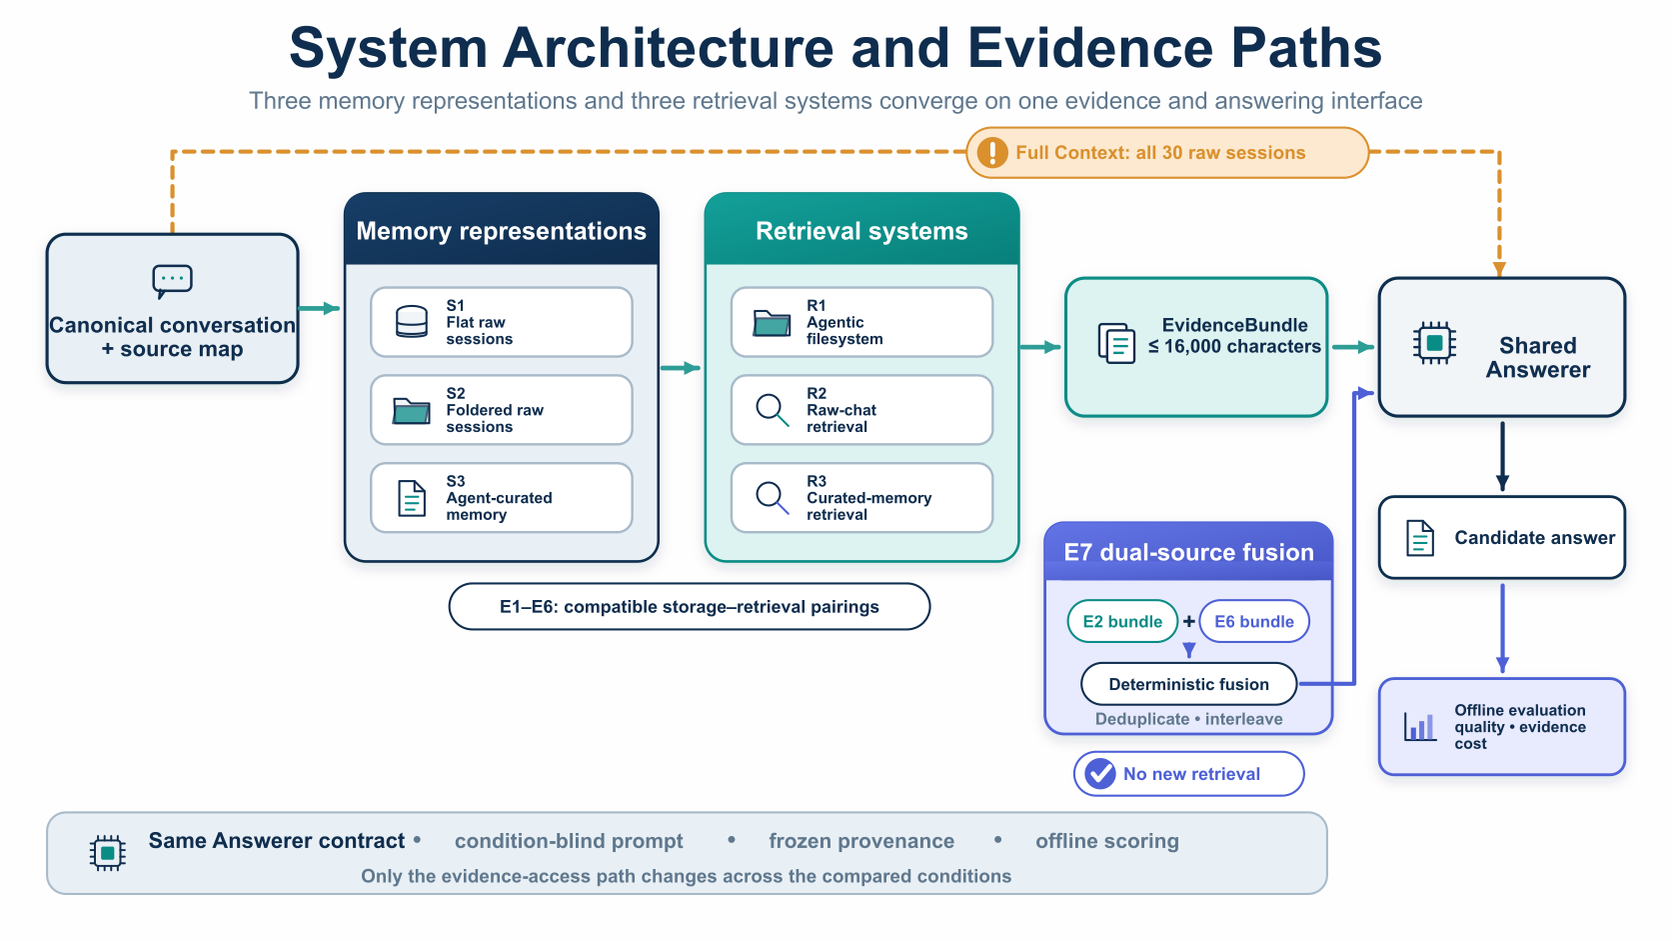
\includegraphics[width=0.68\linewidth,height=0.27\textheight,keepaspectratio]{../figures/chapter-3/figure-3-1-overall-system-architecture.png}
  \caption{Overall system architecture and evidence-access paths. The canonical conversation is transformed into three memory representations and accessed through compatible retrieval systems. Selective conditions converge on a common EvidenceBundle and shared Answerer; E7 fuses the completed E2 and E6 bundles, whereas Full Context bypasses question-dependent retrieval.}
  \label{fig:ch3-1}
\end{figure}

\hypertarget{sec:ch3-4}{%
\section{Data Normalisation and Traceability}\label{sec:ch3-4}}

\hypertarget{sec:ch3-4-1}{%
\subsection{Canonical Source Records}\label{sec:ch3-4-1}}

The study uses one complete conversation selected from the released LoCoMo benchmark \cite{maharana2024locomo}. Local preprocessing verification identifies 30 sessions and converts their contents into one canonical sequence of 568 source-turn records before any memory representation is constructed.

Each canonical record contains:

\begin{itemize}
\tightlist
\item
  the conversation identifier;
\item
  session identifier and session date;
\item
  position within the session;
\item
  global position within the conversation;
\item
  speaker;
\item
  original dialogue text;
\item
  original LoCoMo dialogue identifier;
\item
  a stable project locator;
\item
  an available image caption;
\item
  a content identity.
\end{itemize}

A locator follows the form \([SxTy]\), where \(x\) identifies the session and \(y\) identifies the source turn within that session. For example, \([S3T4]\) denotes the fourth source turn in the third session.

The canonical layer standardises identity and ordering without intentionally rewriting dialogue content. S1, S2, and S3 are derived from this shared layer. Differences among the stores therefore do not result from separate source parsing procedures.

The source contains 30 sessions and 568 source turns. Existing image captions are retained as fixed text when available. The system does not reopen image URLs or run a new vision model. The experiment is therefore based on the textual dialogue and the captions already present in the benchmark source.

\hypertarget{sec:ch3-4-2}{%
\subsection{Raw Session Serialisation}\label{sec:ch3-4-2}}

The canonical records are serialised into one Markdown file per natural session. Within each file, source turns remain in their original order. The serialisation preserves speaker labels, session date, source text, available captions, and stable locators.

These session files form the common textual basis of S1 and S2. S1 places them in one flat directory. S2 moves each complete file into a topic directory. Since the file bodies remain unchanged, any difference between the two raw representations arises from their navigational structure rather than rewritten dialogue.

Session serialisation also preserves natural temporal boundaries. No source turn is moved from one session body to another, and no source turn is duplicated or deleted during construction of the raw stores.

\hypertarget{sec:ch3-4-3}{%
\subsection{Exchange Construction}\label{sec:ch3-4-3}}

R2 requires retrieval units smaller than a full session but broader than one isolated source turn. The system therefore constructs deterministic exchange units within each session.

For session \(\sigma_i\), each complete adjacent pair forms an exchange:

\[
x_{i,j}=(u_{i,2j-1},u_{i,2j}),
\qquad
j\leq\left\lfloor\frac{n_i}{2}\right\rfloor.
\]

Pairing follows the original order:

\[
(T_1,T_2),\ (T_3,T_4),\ (T_5,T_6),\ldots
\]

If \(n_i\) is odd, the final exchange is the singleton:

\[
x_{i,\lceil n_i/2\rceil}=(u_{i,n_i}).
\]

Exchanges never cross a session boundary. Every source turn appears in exactly one exchange.

The 568 source turns produce 292 exchange units across 30 sessions. An exchange is a retrieval unit rather than a summary. Its indexed content is derived directly from the corresponding speakers, source text, and available captions.

This unit provides more local conversational context than one source turn while remaining small enough for lexical ranking and neighbourhood expansion.

\hypertarget{sec:ch3-4-4}{%
\subsection{Source Map and Stable Provenance}\label{sec:ch3-4-4}}

The source map connects the project's canonical identifiers to the original benchmark records. For each locator, it resolves:

\begin{itemize}
\tightlist
\item
  the canonical source-turn record;
\item
  the original LoCoMo dialogue identifier;
\item
  session and date;
\item
  speaker;
\item
  source text;
\item
  available caption.
\end{itemize}

This map creates a common provenance layer for all memory and retrieval paths. It is not supplied to a Retrieval Agent as hidden benchmark information. It is used by the host to verify selected sources and to support later evidence evaluation.

Stable provenance is important because the same source may appear in different forms. In S1 and S2, the source text appears directly in a session file. In S3, one curated fact may restate or combine several source turns. The attached locators preserve a link from that rewritten fact to the canonical source.

\hypertarget{sec:ch3-4-5}{%
\subsection{Traceability across S1, S2, and S3}\label{sec:ch3-4-5}}

Traceability is implemented differently for each representation.

S1 contains the original session text and locator directly. Evidence selected by R1 can therefore be resolved from the observed file and line range. Evidence selected by R2 is resolved from exchange windows whose source turns already have canonical identifiers.

S2 preserves the same file bodies. Its additional directory path changes navigation but not source identity. A source turn therefore retains the same locator and original dialogue identifier in S1 and S2.

S3 contains curated factual units rather than verbatim session records. Each formal fact retains one or more source locators. R1 may select a range of curated text, while R3 selects fact windows. In either case, the locators are parsed and resolved through the common source map.

This design does not imply that S3 contains every source turn. Curation may omit source material. It means that every formal S3 factual unit used as evidence must identify the source records on which it is based. Provenance validity and source coverage are separate properties.

Figure~\ref{fig:ch3-2} illustrates how one original source turn remains traceable across the raw, foldered, exchange-based, and curated representations before becoming a validated EvidenceItem.

\begin{figure}[tbp]
  \centering
  \begin{minipage}{0.68\linewidth}
\begin{Verbatim}[frame=single,fontsize=\tiny]
Original turn
session 7, turn 12
       v
Canonical record: S07:T12
       |--> S1 raw session file
       |--> S2 topic folder / raw session file
       |--> Exchange unit used by R2
       `--> S3 curated fact [source: S07:T12]
                        v
                 Retrieved evidence
                        v
              Validated EvidenceItem
\end{Verbatim}
  \end{minipage}
  \caption{One canonical source turn remains traceable across raw, foldered, exchange-based, and curated representations.}
  \label{fig:ch3-2}
\end{figure}

\hypertarget{sec:ch3-4-6}{%
\subsection{Conceptual Integrity Requirements}\label{sec:ch3-4-6}}

The normalised data and provenance layer must satisfy several requirements.

First, every raw source turn must resolve to one canonical record. Second, S2 must preserve the contents and source identities of the corresponding S1 session files. Third, every formal factual unit in S3 must contain valid provenance. Fourth, every EvidenceItem must resolve to the declared memory representation and its underlying canonical records. Fifth, missing or invalid provenance cannot be silently reconstructed from model output. Finally, reference answers, gold evidence, question categories, and evaluation labels remain outside the online memory pipeline.

These requirements make it possible to compare representations that differ substantially in structure while retaining a common source basis. They also support the later distinction between information that was absent from a store, information that was present but unretrieved, and information that reached the Answerer but was not used correctly.

\hypertarget{sec:ch3-5}{%
\section{Three Storage Representations}\label{sec:ch3-5}}

The three memory stores originate from the same canonical conversation, but they expose the information in different forms. S1 preserves the original sessions in a flat directory. S2 preserves the same session contents but introduces a topic-based directory hierarchy. S3 rewrites the source dialogue into entity- and topic-centred facts. The three stores therefore differ in both the amount and the type of transformation applied before retrieval.

\hypertarget{sec:ch3-5-1}{%
\subsection{S1: Flat Raw Sessions}\label{sec:ch3-5-1}}

S1 is the least transformed memory representation. It contains one Markdown file for each of the 30 conversation sessions. All session files are stored in a single directory. Within each file, source turns remain in their original chronological order. Speaker names, session dates, dialogue text, image captions, and source locators are preserved.

S1 does not add topic folders, summaries, extracted facts, or cross-session consolidation. Its main advantage is source fidelity. A retriever can inspect the original wording and surrounding dialogue without depending on an earlier summarisation decision. Direct source locators also make retrieved evidence straightforward to trace back to the canonical records.

However, source fidelity does not guarantee easy access. Information about the same person, event, or plan may be distributed across many sessions. Repeated descriptions and later corrections can also make the relevant state difficult to identify. S1 therefore provides a raw-filesystem reference representation rather than an assumption that unmodified dialogue is the best memory format.

\hypertarget{sec:ch3-5-2}{%
\subsection{S2: Foldered Raw Sessions}\label{sec:ch3-5-2}}

S2 is constructed from a verified copy of S1. It contains the same 30 session files, but places each complete file under one of four topic folders: \texttt{music-and-performance}, \texttt{photography}, \texttt{travel-and-outdoors}, and \texttt{cars-and-auto-work}. The body of every session file remains byte-identical to its S1 counterpart. Only the relative path changes.

This design isolates the navigation structure as closely as possible. S2 does not summarise a session, split it into new semantic units, or rewrite its dialogue. It instead adds topic labels that a filesystem Retrieval Agent may use when deciding where to search. The contrast between S1 and S2 therefore asks whether directory organisation adds value when the underlying source text remains fixed.

The path information affects the retrievers in different ways. R1 can inspect and navigate the folder hierarchy directly. R2 does not include folder names in its first-stage BM25 text, so the initial lexical ranking remains based on the same dialogue content as in S1. However, relative paths are visible in the returned observations. They may therefore influence a later query produced by the Retrieval Agent.

S2 also has a limitation. A complete session may contain several themes even though it must occupy one directory. Its folder assignment is therefore a navigation cue rather than a complete semantic description of every source turn.

\hypertarget{sec:ch3-5-3}{%
\subsection{S3: Agent-Curated Memory}\label{sec:ch3-5-3}}

S3 is an agent-curated filesystem. Unlike S2, it changes both the organisation and the wording of the stored information. A Management Agent processes the conversation incrementally and maintains persistent Markdown files. It may create files, add or revise facts, group related information, reconcile later updates, and introduce cross-references. This design follows the broad management-agent paradigm of \emph{Filesystem-Based Memory} \cite{zhou2026filesystem}, while the local provenance and validation rules are project-specific.

The frozen S3 store contains two entity-oriented files, one for each main speaker. Each file uses an H1 heading for the entity and H2 headings for topic groups. Factual list items appear under these topics. The store contains 390 locator-bearing fact units under 35 H2 groups. Every formal fact contains one or more source locators that link it back to the canonical conversation records.

A curated fact may combine information from several source turns or sessions. S3 can therefore place facts that were distant in the raw history into one thematic section. It may also express an updated state more directly than the original dialogue. These properties can reduce local dispersion and provide stronger entity and topic cues.

Curation also introduces a new failure surface. The Management Agent may omit a fact, remove a qualifier, merge different entities, flatten a temporal sequence, or retain a stale state. A later retriever cannot recover information that was never written into S3. Furthermore, curation does not necessarily reduce storage size. In this implementation, detailed consolidation and repeated provenance can make curated facts longer than their source fragments. S3 should therefore be understood as a complete agent-curated memory representation, not as a guaranteed compression method.

Figure~\ref{fig:ch3-3} makes the structural differences among S1, S2, and S3 explicit while retaining their common canonical source basis.

\begin{figure}[tbp]
  \centering
  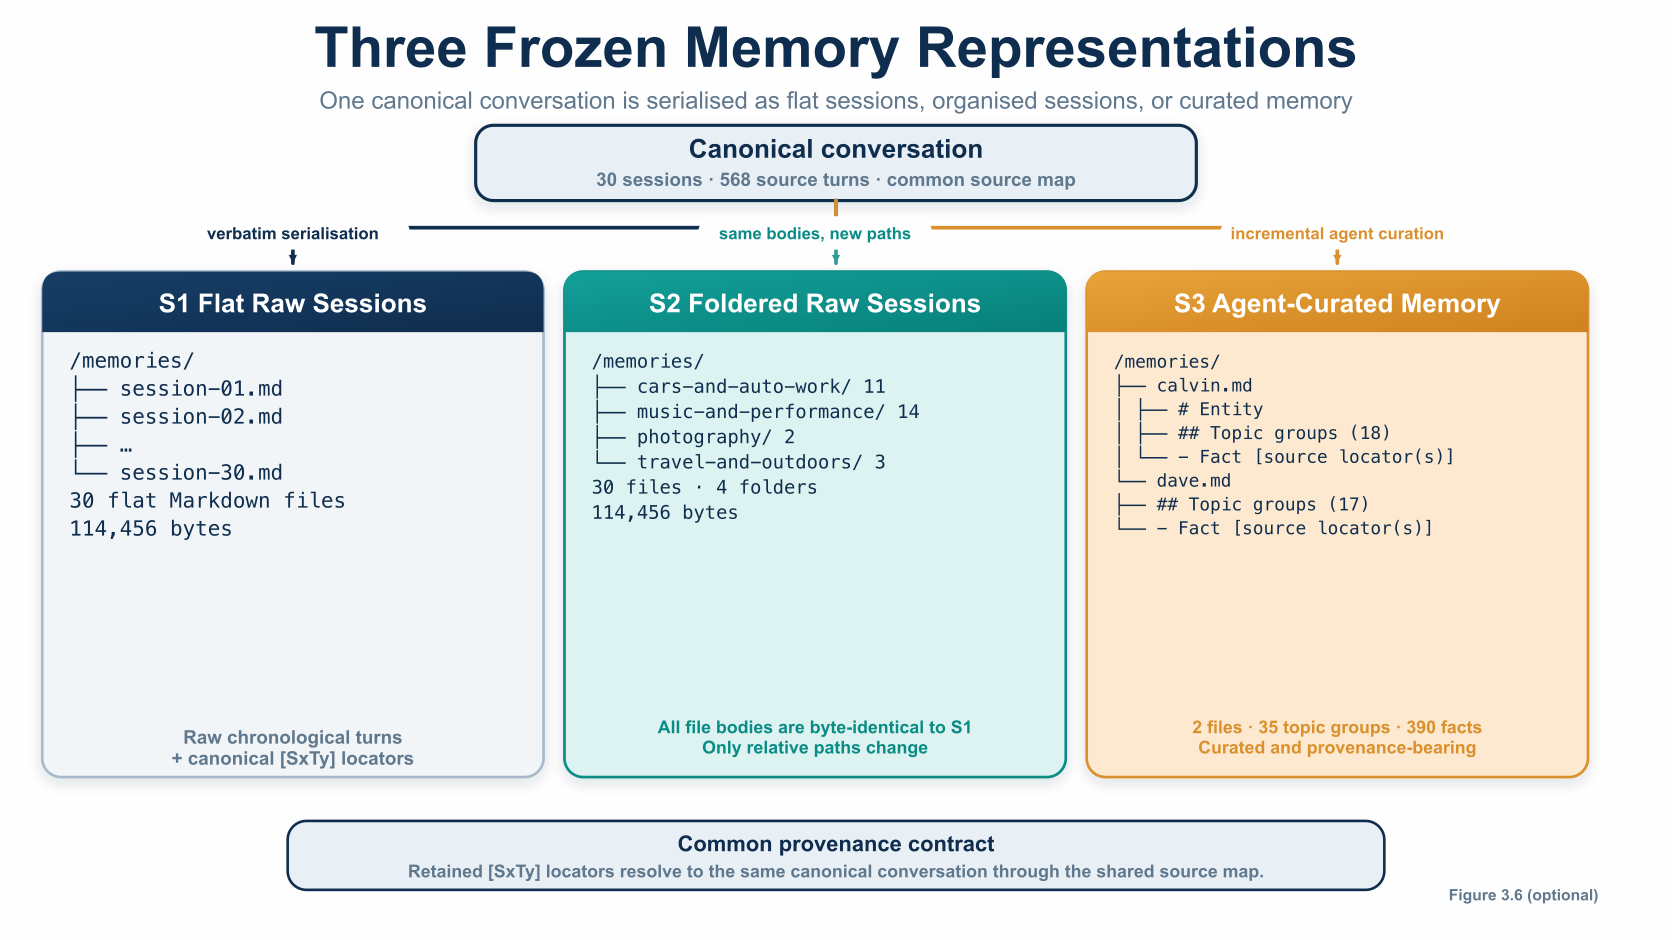
\includegraphics[width=0.68\linewidth,height=0.27\textheight,keepaspectratio]{../figures/chapter-3/figure-3-6-storage-organization.png}
  \caption{Organisation of the three memory representations. S1 stores 30 raw session files in a flat directory; S2 places byte-identical session bodies under four topic folders; S3 reorganises the conversation into two entity files containing 35 topic groups and 390 provenance-bearing facts.}
  \label{fig:ch3-3}
\end{figure}

\setcounter{table}{2}
\begingroup
\renewcommand{\theHtable}{\thechapter.\arabic{table}.block3}
\fontsize{5.0pt}{5.45pt}\selectfont
\setlength{\tabcolsep}{0.7pt}
\renewcommand{\arraystretch}{0.82}
\hfuzz=\maxdimen
\vfuzz=\maxdimen
\begin{longtable}[]{@{}
  >{\raggedright\arraybackslash}p{(.96\columnwidth - 6\tabcolsep) * \real{0.25}}
  >{\raggedright\arraybackslash}p{(.96\columnwidth - 6\tabcolsep) * \real{0.25}}
  >{\raggedright\arraybackslash}p{(.96\columnwidth - 6\tabcolsep) * \real{0.25}}
  >{\raggedright\arraybackslash}p{(.96\columnwidth - 6\tabcolsep) * \real{0.25}}@{}}
\caption[Comparison of the three memory representations.]{Comparison of the three memory representations.}\label{tab:ch3-3}\\
\toprule
Property & S1: Flat Raw Sessions & S2: Foldered Raw Sessions & S3: Agent-Curated Memory \\
\midrule
\endfirsthead
\multicolumn{4}{r}{\small\itshape Continued from the previous page}\\
\toprule
Property & S1: Flat Raw Sessions & S2: Foldered Raw Sessions & S3: Agent-Curated Memory \\
\midrule
\endhead
Primary stored unit & Raw session file & Raw session file & Curated factual item \\
Source wording rewritten & No & No & Yes \\
Main structure & One flat directory & Four topic folders & Entity files and H2 topic groups \\
Chronology & Preserved directly & Preserved directly & Represented through facts, dates, and locators \\
Provenance & Direct source locators & Direct source locators & Inline source locators \\
Main intended benefit & Maximum source fidelity & Additional navigation cues & Thematic grouping and cross-session consolidation \\
Principal risk & Relevant facts remain dispersed & Folder taxonomy may be imperfect & Omission, distortion, or stale consolidation \\
\bottomrule
\end{longtable}
\endgroup

\hypertarget{sec:ch3-6}{%
\section{Three Retrieval Systems}\label{sec:ch3-6}}

R1, R2, and R3 are evidence-retrieval systems. They do not generate the final benchmark answer. Each retriever observes a question, searches one declared memory representation, and selects evidence. The selected material is then validated and converted into the common EvidenceBundle described in Section~\ref{sec:ch3-7}.

\hypertarget{sec:ch3-6-1}{%
\subsection{R1: Agentic Filesystem Retrieval}\label{sec:ch3-6-1}}

R1 is an LLM-controlled filesystem Retrieval Agent based on the filesystem-search paradigm in \cite{zhou2026filesystem}. It receives the question, store-specific search instructions, and read-only access to one mounted memory store. Its role is to locate supporting source material rather than answer the question.

The Agent can use four filesystem tools:

\begin{itemize}
\tightlist
\item
  \texttt{view}, which inspects a file or directory;
\item
  \texttt{grep}, which finds text matches across files;
\item
  \texttt{toc}, which exposes headings and document structure;
\item
  \texttt{section\_read}, which reads a selected document section.
\end{itemize}

These tools provide access but do not determine the search strategy. In particular, \texttt{grep} performs deterministic text matching. The Agent must decide which words or expressions to search, which files require inspection, and whether the returned context is sufficient.

A typical R1 episode follows an observation--action loop. The Agent first surveys the available store. It then formulates a search direction, calls one or more read-only tools, inspects the returned observations, and refines its search when evidence remains incomplete. This process continues until the Agent saves sufficient evidence or reaches a stopping condition.

One accepted action-bearing provider completion is defined as one R1 retrieval round. A completion may request several independent filesystem reads, so one round is not equivalent to one tool call. However, every accepted round must use exactly one action mode: filesystem operations, \texttt{take\_note}, or \texttt{finish\_search}. These modes cannot be mixed in one completion. Evidence selection and search termination therefore consume rounds of their own. Protocol-correction attempts and context-compaction calls are counted separately and do not create retrieval rounds. Store-specific round limits are reported in Chapter~\ref{chap:ch4}.

R1 adds two host-side orchestration actions to the four filesystem tools. These actions are project-specific and are not tools proposed by \emph{Filesystem-Based Memory} \cite{zhou2026filesystem}.

The first action, \texttt{take\_note}, records an evidence selection. The Agent may identify only line ranges that have already appeared in a successful observation. It cannot supply a rewritten quotation or model-generated summary as evidence. The host reopens the frozen file, verifies that the selected range was observed, extracts the exact text, resolves its source locators, and creates an EvidenceItem.

The second action, \texttt{finish\_search}, terminates the retrieval episode. It carries a structured stopping reason, but it cannot contain an answer or introduce new evidence. Its purpose is to close retrieval and hand the validated EvidenceBundle to the downstream Answerer. Thus:

\[
\texttt{finish\_search}\neq\text{answer generation}.
\]

R1 uses different routing guidance for the three store shapes. On S1, the Agent searches a flat collection of raw sessions. On S2, it can use topic folders before inspecting the original session text. On S3, it navigates entity files and topic sections. The underlying filesystem capability remains read-only in all three cases.

\hypertarget{sec:ch3-6-2}{%
\subsection{R2: ReFind-Style Raw-Chat Retrieval}\label{sec:ch3-6-2}}

R2 is an iterative lexical retrieval system for raw dialogue. It adapts the ReFind search principle \cite{li2026refind} to the canonical exchange units defined in Section~\ref{sec:ch3-4}. The local exchange is the functional counterpart of ReFind's paired dialogue turn, not the single-speaker LoCoMo source-turn unit. Its retrieval hierarchy is:

\[
\text{exchange}\rightarrow\text{session}.
\]

An exchange is the first-stage scoring unit, while a session is the higher-level grouping unit. R2 operates over 292 exchanges derived from the 568 source turns in the 30-session conversation.

At each search step, the Retrieval Agent generates one lexical query and may also specify a date range. The query is tokenised and scored jointly against every eligible exchange. R2 does not automatically execute a separate search for each query word.

The indexed exchange text includes speaker names, original dialogue, and available image captions. It excludes gold information and experimental labels. Source locators and folder paths are retained for provenance but do not contribute lexical ranking terms.

R2 first assigns a BM25 score to each eligible exchange \cite{robertson2009bm25}. Positive exchange scores are then aggregated within each session to produce a session-level score. Each exchange consequently receives both an exchange rank and the rank of its parent session. The two views are combined by Reciprocal Rank Fusion \cite{cormack2009rrf}:

\[
\operatorname{RRF}(x)=
\frac{1}{60+r_x}
+
\frac{1}{60+r_{\sigma(x)}},
\]

where \(r_x\) is the exchange rank and \(r_{\sigma(x)}\) is the rank of its parent session. The system returns the five highest-ranked centre exchanges.

A centre exchange is not presented in isolation. It is expanded with up to two preceding and two following exchanges from the same session. Expansion never crosses a session boundary. This local window provides the Retrieval Agent with nearby speaker and event context that may not share the query terms.

R2 also maintains a seen-session state. Once a session appears in a search result, that session is excluded from later searches in the same question episode. This rule encourages the Agent to inspect new parts of the conversation rather than repeatedly retrieve the same session.

The controller supports three actions:

\begin{enumerate}
\def\labelenumi{\arabic{enumi}.}
\tightlist
\item
  \texttt{search\_chatrecord};
\item
  \texttt{take\_note};
\item
  \texttt{finish\_search}.
\end{enumerate}

Each of the four permitted provider completions may produce one valid action. Search, evidence selection, and stopping all consume this same cap. A valid four-completion episode therefore does not necessarily contain four searches. A malformed or empty completion also consumes one completion even though it produces no accepted action.

When the Agent selects a returned context block, the host reopens the raw store and resolves the block to canonical source turns. Overlapping selections are merged deterministically, duplicated source turns are removed, and provenance is validated before an EvidenceItem enters the EvidenceBundle. Model-written text cannot replace the source evidence.

R2 uses the same dialogue text for S1 and S2. Their initial backend ranking is therefore identical for the same query. Later behaviour may differ because S2 paths are visible in observations and can influence subsequent query reformulation. This distinction allows E2 and E4 to test whether folder cues affect an iterative retrieval process even when they are excluded from first-stage lexical scoring.

\hypertarget{sec:ch3-6-3}{%
\subsection{R3: Retrieval Adapted to Curated Memory}\label{sec:ch3-6-3}}

R3 adapts the main R2 retrieval pattern \cite{li2026refind} to the structure of S3. It is not a third algorithm proposed by ReFind. The appropriate description is \textbf{ReFind-inspired retrieval over agent-curated memory}.

R2 cannot be applied unchanged to S3 because S3 does not consist of raw exchanges grouped by sessions. Its retrieval hierarchy is instead:

\[
\text{curated fact}\rightarrow\text{H2 topic group}.
\]

The frozen S3 index contains 390 locator-bearing fact units under 35 H2 topic groups. YAML front matter is excluded because it provides file-level description rather than factual evidence.

Each fact is indexed using three components: the entity name, the H2 topic heading, and the fact text with source-locator syntax removed. Entity and topic terms allow S3's organisation to contribute to lexical retrieval. The separately stored relative-path and source-locator metadata do not become ranking terms. However, a literal cross-reference path written inside the curated fact remains part of the fact text and can affect lexical scoring.

R3 assigns a BM25 score to each eligible fact \cite{robertson2009bm25}. Positive fact scores are aggregated within their H2 groups. Fact rank and topic-group rank are then combined using the same Reciprocal Rank Fusion formula as R2 \cite{cormack2009rrf}. The five highest-ranked centre facts are returned.

Each centre fact is expanded with up to two neighbouring facts in the same H2 section. Expansion cannot cross an H2 or file boundary. This restriction preserves the thematic context created during memory construction.

R3 tracks seen H2 groups rather than seen sessions. Once a topic group appears in a result, that group is excluded from later searches in the same episode. Other topics for the same entity remain eligible. This is important because one entity file may contain many distinct topic groups.

Temporal filtering also requires an adaptation. A raw exchange belongs to one session date, whereas one curated fact may cite several source turns from different dates. R3 resolves all source dates through the fact's locators. A centre fact is eligible for ranking when at least one of these dates overlaps the requested interval. The subsequent \(\pm2\) neighbourhood expansion preserves local topic context and does not reapply the date predicate, so a neighbouring fact may lie outside the requested interval.

The controller retains the same three-action interface and four-completion cap as R2: \texttt{search\_chatrecord}, \texttt{take\_note}, and \texttt{finish\_search}. Invalid completions also consume the cap. When the Agent selects a result, the host reopens the frozen S3 file, verifies the fact range and H2 boundary, parses its locators, resolves the corresponding canonical records, and constructs the EvidenceItem.

R3 can improve access to information that exists in S3, but it cannot repair a write omission. It is also sensitive to the structure created during curation. Very large topic groups may receive stronger aggregate scores, and a long curated fact may introduce more material than the question requires. These properties form part of the retrieval mechanism rather than evidence of superior or inferior performance.

Figure~\ref{fig:ch3-4} compares the control flow of the three retrieval systems and their common handoff boundary.

\begin{figure}[tbp]
  \centering
  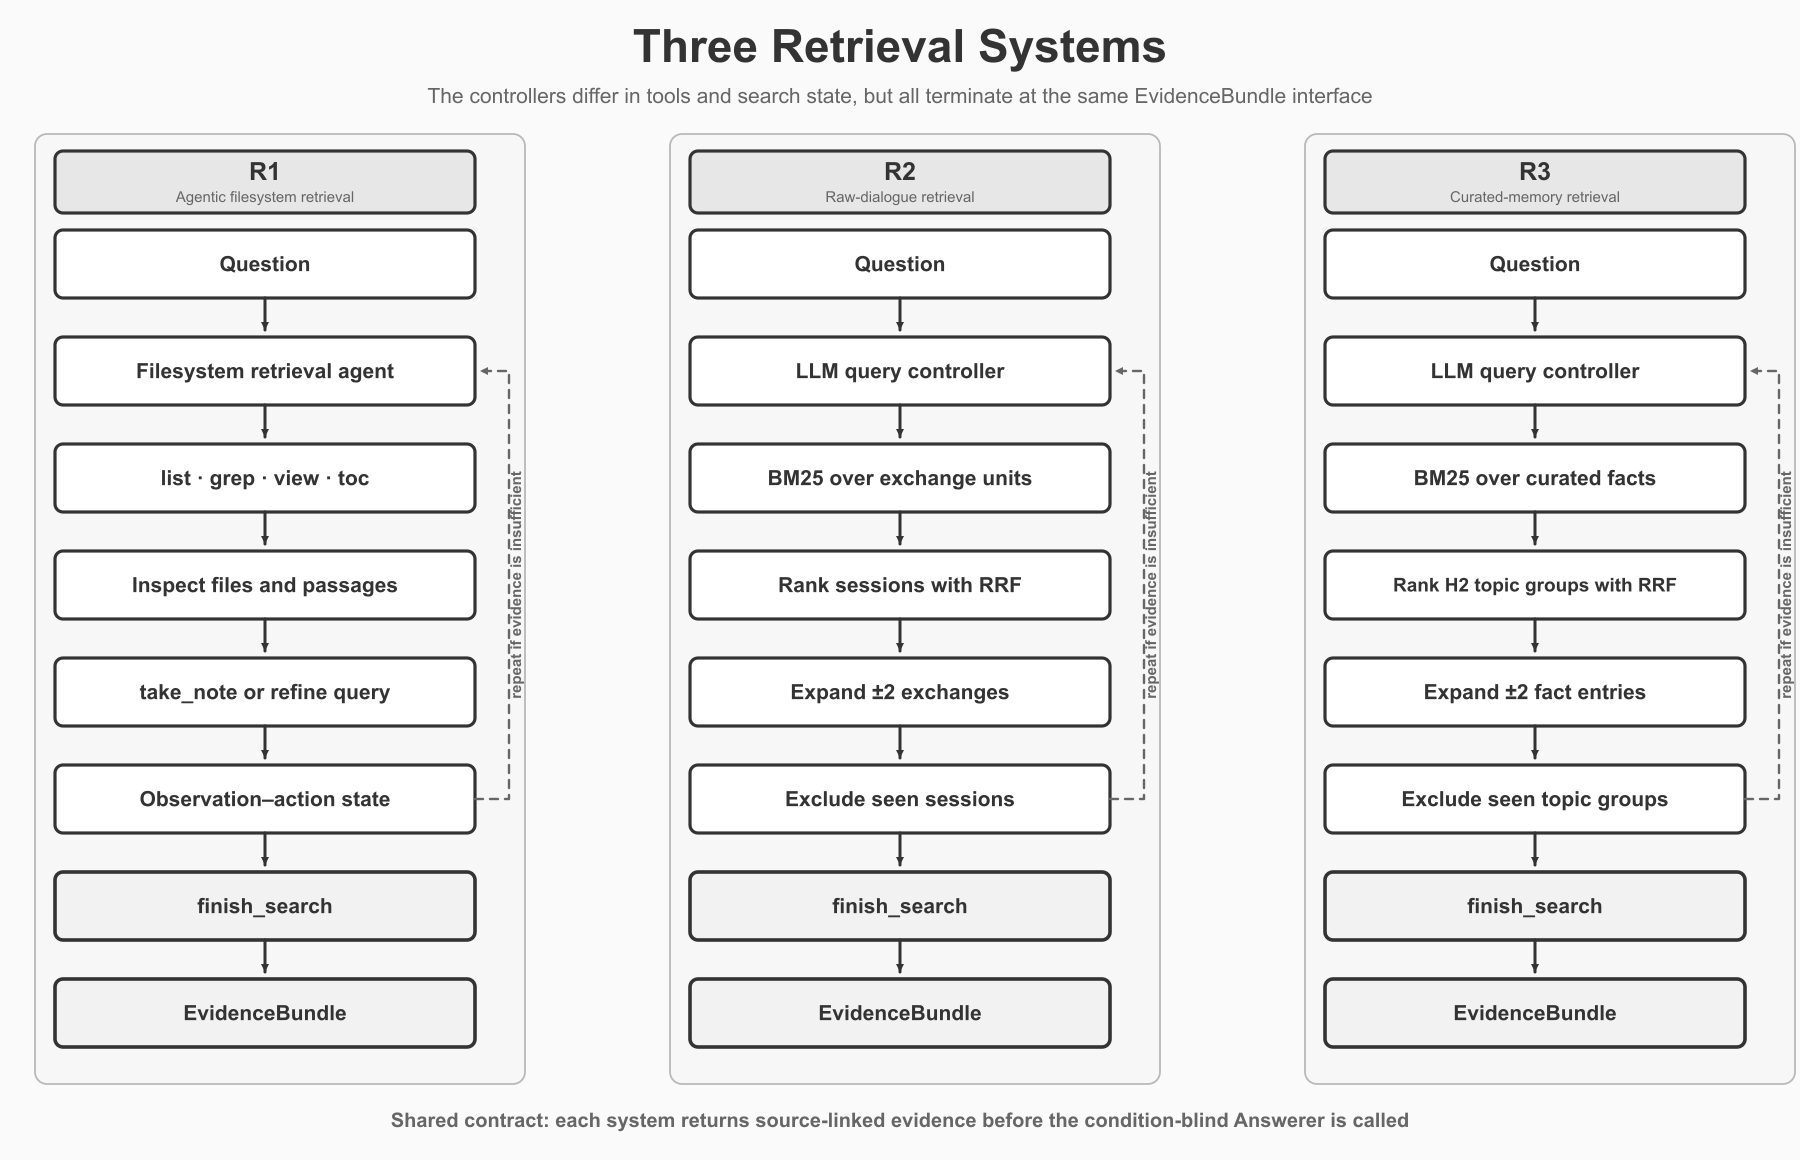
\includegraphics[width=0.62\linewidth,height=0.32\textheight,keepaspectratio]{../figures/chapter-3/figure-3-3-retrieval-system-flowcharts.png}
  \caption{Control flow of R1, R2, and R3. R1 navigates a read-only filesystem through iterative observations and actions, R2 ranks raw exchanges and expands within sessions, and R3 ranks curated facts and expands within H2 topic groups. Each path terminates retrieval through \texttt{finish\_search} and returns a validated EvidenceBundle rather than a benchmark answer.}
  \label{fig:ch3-4}
\end{figure}

\setcounter{table}{3}
\begingroup
\renewcommand{\theHtable}{\thechapter.\arabic{table}.block4}
\fontsize{5.0pt}{5.45pt}\selectfont
\setlength{\tabcolsep}{0.7pt}
\renewcommand{\arraystretch}{0.82}
\hfuzz=\maxdimen
\vfuzz=\maxdimen
\begin{longtable}[]{@{}
  >{\raggedright\arraybackslash}p{(.96\columnwidth - 6\tabcolsep) * \real{0.25}}
  >{\raggedright\arraybackslash}p{(.96\columnwidth - 6\tabcolsep) * \real{0.25}}
  >{\raggedright\arraybackslash}p{(.96\columnwidth - 6\tabcolsep) * \real{0.25}}
  >{\raggedright\arraybackslash}p{(.96\columnwidth - 6\tabcolsep) * \real{0.25}}@{}}
\caption[Comparison of the three retrieval systems.]{Comparison of the three retrieval systems.}\label{tab:ch3-4}\\
\toprule
Property & R1 & R2 & R3 \\
\midrule
\endfirsthead
\multicolumn{4}{r}{\small\itshape Continued from the previous page}\\
\toprule
Property & R1 & R2 & R3 \\
\midrule
\endhead
Formal name & Agentic Filesystem Retrieval & ReFind-Style Raw-Chat Retrieval & Retrieval Adapted to Curated Memory \\
Compatible stores & S1, S2, and S3 & S1 and S2 & S3 \\
Main retrieval unit & File region or section & Raw exchange & Curated fact \\
Higher-level group & Filesystem path or section & Session & H2 topic group \\
Search mechanism & Agent-controlled filesystem tools & BM25, session aggregation, and RRF & BM25, topic aggregation, and RRF \\
Local context & Agent-selected reads & Up to \(\pm2\) exchanges within one session & Up to \(\pm2\) facts within one H2 group \\
Seen-state & No explicit backend exclusion state; prior observations remain in the trace & Previously returned sessions & Previously returned H2 groups \\
Evidence selection & Observed line ranges & Returned exchange windows & Returned fact windows \\
Stopping mechanism & \texttt{finish\_search} or round limit & \texttt{finish\_search} or action limit & \texttt{finish\_search} or action limit \\
Principal limitation & Tool-use cost and behavioural variation & Query mismatch or missed implicit relations & Dependence on S3 content and topic structure \\
\bottomrule
\end{longtable}
\endgroup

\hypertarget{sec:ch3-7}{%
\section{Shared EvidenceBundle and Answerer}\label{sec:ch3-7}}

The retrieval systems differ internally, but their outputs must reach the Answerer through a common interface. Otherwise, an apparent retrieval effect could instead be caused by a different evidence format or answering prompt. All selective conditions therefore convert their selected material into the same EvidenceBundle schema.

\hypertarget{sec:ch3-7-1}{%
\subsection{Retrieval-Neutral Evidence Interface}\label{sec:ch3-7-1}}

An EvidenceBundle is an ordered collection of validated EvidenceItems associated with one question and one condition. It hides retriever-specific control details from the Answerer while preserving the text and provenance required for answering.

R1 contributes observed filesystem ranges, R2 contributes raw exchange windows, and R3 contributes curated fact windows. These internal units remain visible in the retrieval record, but the Answerer receives them through one common item format. Retrieval scores, search queries, tool observations, and stopping reasons are not part of the answering input.

\hypertarget{sec:ch3-7-2}{%
\subsection{EvidenceItem Structure}\label{sec:ch3-7-2}}

Each EvidenceItem contains:

\begin{itemize}
\tightlist
\item
  a stable evidence identifier;
\item
  the exact selected text;
\item
  the source kind;
\item
  the source path or structural group;
\item
  source locators;
\item
  canonical source-record identifiers;
\item
  source dates and speakers where applicable;
\item
  selection order; and
\item
  a deterministic content identity.
\end{itemize}

This schema preserves two levels of provenance. The representation-level fields identify where the evidence was read, such as a raw session path or a curated topic group. The canonical fields identify the underlying source turns. Both are required because a curated fact may differ in wording from the source records on which it is based.

\hypertarget{sec:ch3-7-3}{%
\subsection{Evidence Validation}\label{sec:ch3-7-3}}

The Retrieval Agent chooses evidence references rather than authoring evidence text. For R1, it selects previously observed file ranges. For R2 and R3, it selects returned result blocks. The host then reopens the declared frozen store and reconstructs the evidence from source bytes.

This validation boundary prevents a model-generated paraphrase from being treated as retrieved evidence. It also ensures that every source locator resolves through the common provenance layer. Invalid, unobserved, or unresolvable selections are rejected rather than silently repaired.

\hypertarget{sec:ch3-7-4}{%
\subsection{Evidence Ordering, Merging, and Budget}\label{sec:ch3-7-4}}

EvidenceItems retain a deterministic order derived from their accepted selections. Same-path selections with identical, contained, overlapping, or adjacent source ranges may be rejected or merged when the provenance permits it. Repeated anchors are also rejected in R2 and R3. Identical text at two distinct provenance locations is not globally deduplicated.

Each single-source condition from E1 to E6 uses a maximum evidence budget of:

\[
\beta=16{,}000\text{ characters}.
\]

The budget is applied after deterministic evidence merging. Complete EvidenceItems are retained or skipped; their text is not silently cut in the middle. This common limit prevents one selective retriever from obtaining a larger Answerer input simply because it emits more evidence. Chapter~\ref{chap:ch4} treats the budget as a fixed experimental control.

\hypertarget{sec:ch3-7-5}{%
\subsection{Shared Answerer Input}\label{sec:ch3-7-5}}

The Answerer receives the question, the ordered EvidenceBundle, and the shared answering instructions. Its prompt presents evidence through stable identifiers so that the generated answer can cite the supplied material. The Answerer has no retrieval tools and cannot request more memory after the bundle has been finalised.

Full Context uses the same Answerer renderer, answer-generation objective, and structured response contract. To reuse this interface, the 30 complete S1 session bodies are wrapped as 30 content-addressed EvidenceItems in a non-selective full-context bundle. The Answerer therefore cites ordinary evidence identifiers. What Full Context bypasses is question-dependent retrieval and the selective 16,000-character budget, not evidence packaging or citation validation.

\hypertarget{sec:ch3-7-6}{%
\subsection{Condition-Blind Answering}\label{sec:ch3-7-6}}

The Answerer does not receive the condition identifier, store label, retriever name, retrieval trace, retrieval scores, gold answer, gold evidence, or evaluation labels. It is therefore blind to the explicit condition label. It is not blind to evidence provenance: the rendered items expose source kind, text, timestamps, and locators. In E7, the presence of both raw and curated items is consequently visible even though the label ``E7'' is not.

This condition-label-blind boundary keeps answer generation comparable. E1--E7 may change the memory path and the evidence delivered, but they do not change the role of the Answerer. Any remaining difference enters through the evidence content and provenance or through stochastic model behaviour, not through an explicit condition instruction.

\hypertarget{sec:ch3-7-7}{%
\subsection{Output Contract}\label{sec:ch3-7-7}}

The Answerer returns a structured object with three fields:

\begin{itemize}
\tightlist
\item
  \texttt{answer};
\item
  \texttt{citations};
\item
  \texttt{insufficient\_evidence}.
\end{itemize}

A citation may refer only to an evidence identifier present in the input bundle. The \texttt{insufficient\_evidence} field records whether the Answerer judges the supplied evidence to be inadequate. It does not trigger another retrieval attempt.

If the initial response violates the output schema, the system may perform a constrained format repair. The repair cannot retrieve new material or change the EvidenceBundle. Its prompt instructs the model to preserve the answer content, use only allowed evidence identifiers, and add no new facts or citations. The purpose is to recover a valid representation of the original response; the repair is not treated as another retrieval or answering stage.

Figure~\ref{fig:ch3-5} summarises the validation, packaging, and answering boundary shared by the selective conditions.

\begin{figure}[tbp]
  \centering
  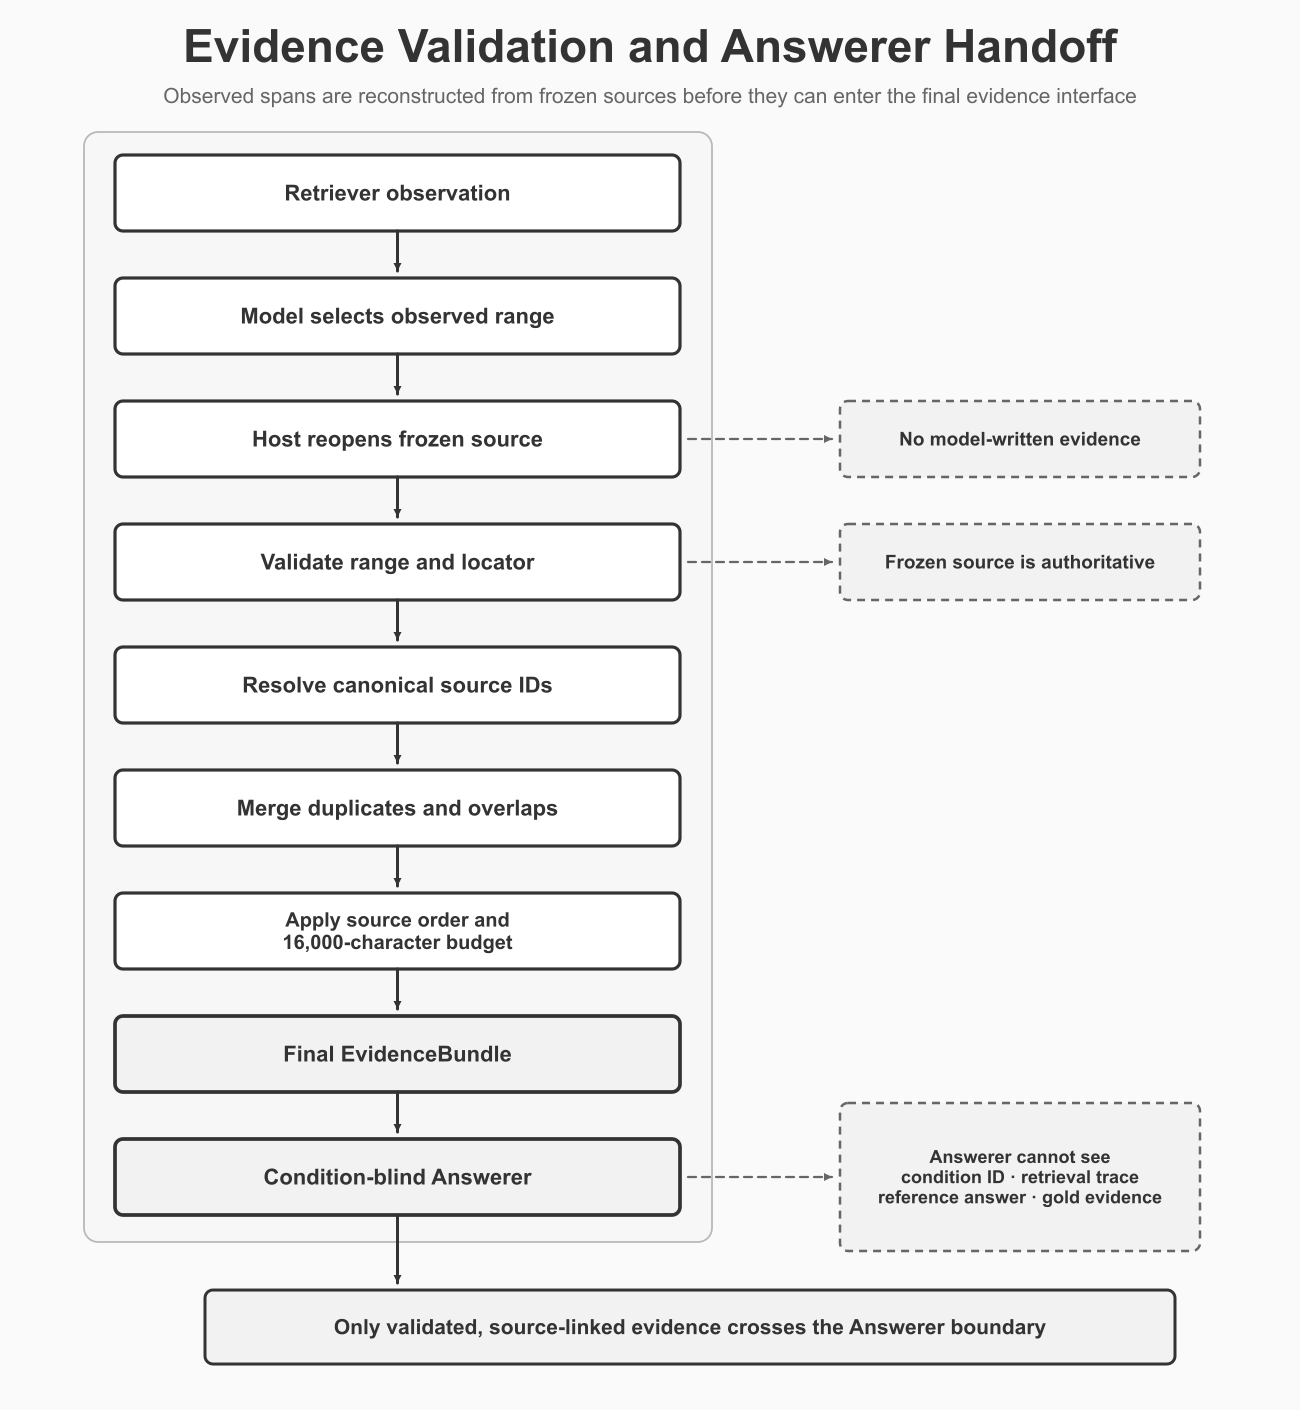
\includegraphics[width=0.54\linewidth,height=0.30\textheight,keepaspectratio]{../figures/chapter-3/figure-3-4-evidence-validation-and-answerer.png}
  \caption{Evidence validation and Answerer handoff. Model-selected evidence references are resolved against frozen source bytes, validated, ordered, merged, and budgeted before the condition-blind Answerer generates a structured candidate response.}
  \label{fig:ch3-5}
\end{figure}

\hypertarget{sec:ch3-8}{%
\section{Mapping of E1--E7 Conditions}\label{sec:ch3-8}}

\hypertarget{sec:ch3-8-1}{%
\subsection{Complete Condition Map}\label{sec:ch3-8-1}}

The seven experimental conditions describe complete paths from a memory representation to the shared Answerer. They are not seven independent retrieval algorithms.

\setcounter{table}{4}
\begingroup
\renewcommand{\theHtable}{\thechapter.\arabic{table}.block5}
\fontsize{5.0pt}{5.45pt}\selectfont
\setlength{\tabcolsep}{0.7pt}
\renewcommand{\arraystretch}{0.82}
\hfuzz=\maxdimen
\vfuzz=\maxdimen
\begin{longtable}[]{@{}
  >{\raggedright\arraybackslash}p{(.96\columnwidth - 8\tabcolsep) * \real{0.20}}
  >{\raggedright\arraybackslash}p{(.96\columnwidth - 8\tabcolsep) * \real{0.20}}
  >{\raggedright\arraybackslash}p{(.96\columnwidth - 8\tabcolsep) * \real{0.20}}
  >{\raggedright\arraybackslash}p{(.96\columnwidth - 8\tabcolsep) * \real{0.20}}
  >{\raggedright\arraybackslash}p{(.96\columnwidth - 8\tabcolsep) * \real{0.20}}@{}}
\caption[Storage, retrieval, and evidence composition of E1--E7.]{Storage, retrieval, and evidence composition of E1--E7.}\label{tab:ch3-5}\\
\toprule
Condition & Memory representation or source & Retrieval or processing & Evidence supplied to the Answerer & Primary methodological role \\
\midrule
\endfirsthead
\multicolumn{5}{r}{\small\itshape Continued from the previous page}\\
\toprule
Condition & Memory representation or source & Retrieval or processing & Evidence supplied to the Answerer & Primary methodological role \\
\midrule
\endhead
E1 & S1: Flat Raw Sessions & R1 & Raw filesystem spans & Flat raw-filesystem reference path \\
E2 & S1: Flat Raw Sessions & R2 & Ranked raw exchange windows & Enhanced retrieval over flat raw dialogue \\
E3 & S2: Foldered Raw Sessions & R1 & Raw filesystem spans & Effect of directory organisation on R1 \\
E4 & S2: Foldered Raw Sessions & R2 & Ranked raw exchange windows & Interaction between folder cues and R2 \\
E5 & S3: Agent-Curated Memory & R1 & Curated filesystem spans & General filesystem retrieval over curated memory \\
E6 & S3: Agent-Curated Memory & R3 & Ranked curated fact windows & Retrieval adapted to curated structure \\
E7 & E2 and E6 EvidenceBundles & Deterministic fusion & Interleaved raw and curated evidence & Dual-source complementarity and interference \\
\bottomrule
\end{longtable}
\endgroup

\hypertarget{sec:ch3-8-2}{%
\subsection{Controlled Raw-Memory Core}\label{sec:ch3-8-2}}

E1--E4 form the controlled raw-memory core. E1 and E2 share S1 but use different retrieval systems. E3 and E4 share S2 but use different retrieval systems. E1 and E3 use R1 over the same raw session contents under different directory structures. E2 and E4 apply R2 to the same raw exchange corpus while exposing different provenance paths in the observations.

These relations support the closest component-level comparisons in the study. They distinguish the effect of directory organisation from the effect of the retrieval family without changing the underlying dialogue.

\hypertarget{sec:ch3-8-3}{%
\subsection{Curated-Memory Extension}\label{sec:ch3-8-3}}

E5 and E6 use the same frozen S3 snapshot. E5 asks a general filesystem Agent to navigate curated files and sections. E6 applies retrieval that is explicitly adapted to S3's fact and topic structure.

These conditions compare access methods over the same curated store. Comparisons between E5 or E6 and raw-store conditions are broader system comparisons. S3 changes wording, granularity, organisation, and the presentation of provenance, so such comparisons cannot be interpreted as a single-feature storage ablation.

\hypertarget{sec:ch3-8-4}{%
\subsection{Dual-Source Condition}\label{sec:ch3-8-4}}

E7 is constructed from the completed E2 and E6 EvidenceBundles. It does not add another memory representation or retrieval system. Its purpose is to test whether already selected raw and curated evidence provide complementary information or create interference when presented together.

The parent pair is methodologically meaningful. E2 supplies evidence from raw dialogue through the retrieval system designed for raw chat. E6 supplies evidence from curated memory through the adapter designed for curated facts. Their fusion therefore contrasts two complete, representation-appropriate evidence paths.

\hypertarget{sec:ch3-8-5}{%
\subsection{Interpretation Boundaries}\label{sec:ch3-8-5}}

The condition set is theory-driven rather than an exhaustive Cartesian product. R3 is a representation-specific adaptation of the R2 retrieval principle, not a universal retriever that must be paired with every store. E7 is a fusion condition, not a new retrieval algorithm. Full Context is a diagnostic path outside E1--E7.

The strength of an inference also depends on the comparison. E1 versus E3 and E2 versus E4 isolate directory organisation most directly because the raw file contents are held constant. E1 versus E2, E3 versus E4, and E5 versus E6 compare retrieval systems on one fixed store. Comparisons between raw and curated conditions concern complete system paths because curation changes several properties at once.

Replicating the same condition graph with another backbone model does not create new E-condition definitions. It tests whether the observed effects remain stable when the model changes.

\hypertarget{sec:ch3-9}{%
\section{Alternative Evidence-Access Paths}\label{sec:ch3-9}}

E7 and Full Context depart from the standard single-store selective path in different ways. E7 retains selective retrieval but combines two completed evidence sources. Full Context removes external evidence selection and sends the complete raw conversation to the Answerer.

\hypertarget{sec:ch3-9-1}{%
\subsection{E7 Dual-Source Fusion}\label{sec:ch3-9-1}}

E7 requires a completed E2 EvidenceBundle and a completed E6 EvidenceBundle for the same question. The two parent bundles represent different evidence sources:

\begin{itemize}
\tightlist
\item
  E2 provides raw dialogue evidence selected through R2;
\item
  E6 provides curated facts selected through R3.
\end{itemize}

Before fusion, the system verifies that both bundles correspond to the same question and the expected parent conditions. Their provenance and single-source budgets must also remain valid. If either parent is missing or mismatched, E7 is not produced.

Fusion is deterministic. The order inside each parent bundle is preserved, while the two streams are interleaved:

\[
\text{raw}_1,\ \text{curated}_1,
\text{raw}_2,\ \text{curated}_2,\ldots
\]

This rule prevents one source from occupying the entire beginning of the Answerer input.

Exact duplicates are identified using the combination of source kind, canonical source identifiers, and evidence-text identity:

\[
(\text{source kind},\ \text{source identifiers},\ \text{text hash}).
\]

Source kind remains part of the key because raw and curated items may cite the same source turns while expressing them differently. Such items are retained when their text differs. This allows E7 to preserve the distinction between original dialogue and its curated representation.

Each parent bundle retains the single-source budget:

\[
|\mathcal{B}_{E2}|\leq\beta,
\qquad
|\mathcal{B}_{E6}|\leq\beta.
\]

The fused evidence is therefore bounded by:

\[
|\mathcal{B}_{E7}|\leq2\beta
=32{,}000\text{ characters}.
\]

The fused bundle is then passed to the shared Answerer once. Fusion does not formulate a query, rerun R1, R2, or R3, invoke an LLM, or create an intermediate summary. E7 therefore measures post-retrieval complementarity and interference rather than the performance of a new joint retriever.

\hypertarget{sec:ch3-9-2}{%
\subsection{Full Context Diagnostic Path}\label{sec:ch3-9-2}}

Full Context uses a separate evidence-access path. For each question, it constructs one deterministic input containing all 30 raw sessions and all 568 source turns. Sessions and turns remain in fixed chronological order. Original dialogue and available image captions are retained. No question-dependent filtering, summarisation, or reordering is performed.

The Full Context answer can be represented as:

\[
\hat{a}_{FC}=A_\theta(q,\mathcal{C}),
\]

where \(\mathcal{C}\) is the complete canonical raw conversation. In contrast, a selective condition uses:

\[
\hat{a}=A_\theta(q,\mathcal{B}),
\]

where \(\mathcal{B}\) is a question-specific EvidenceBundle.

Full Context does not use S2, S3, R1, R2, R3, or E7 fusion. It packages the 30 complete S1 session bodies as a non-selective full-context bundle so that it can use the shared Answerer interface. It does not apply the 16,000-character selective-evidence limit. Applying that limit would convert it into a truncated-context condition rather than Full Context.

The Answerer retains the same answer-generation objective and structured output contract where applicable. The principal change is the information-access path: the model must locate and combine relevant information inside the complete history instead of receiving externally selected evidence.

Full Context is a diagnostic path, not a fourth memory store, a fourth retriever, or an eighth E-condition. It is also not a theoretical oracle. Complete visibility does not ensure correct use, and long-context performance can depend on evidence position \cite{liu2024lost}. The Answerer may still be affected by repeated facts, changing states, entity similarity, temporal confusion, or failed multi-session composition.

The comparison is informative in both directions. If Full Context repairs a selective-retrieval error, missing evidence is a plausible explanation. If selective retrieval succeeds while Full Context fails, evidence reduction may have improved focus. If both paths receive the required information but fail, the remaining difficulty is more likely to involve evidence utilisation or reasoning \cite{yuan2026retrievalutilization}. Chapter~\ref{chap:ch4} defines how these paths are evaluated, and Chapter~\ref{chap:ch5} examines their observed behaviour.

Figure~\ref{fig:ch3-6} contrasts the two alternative evidence-access paths while holding the answering objective constant.

\begin{figure}[tbp]
  \centering
  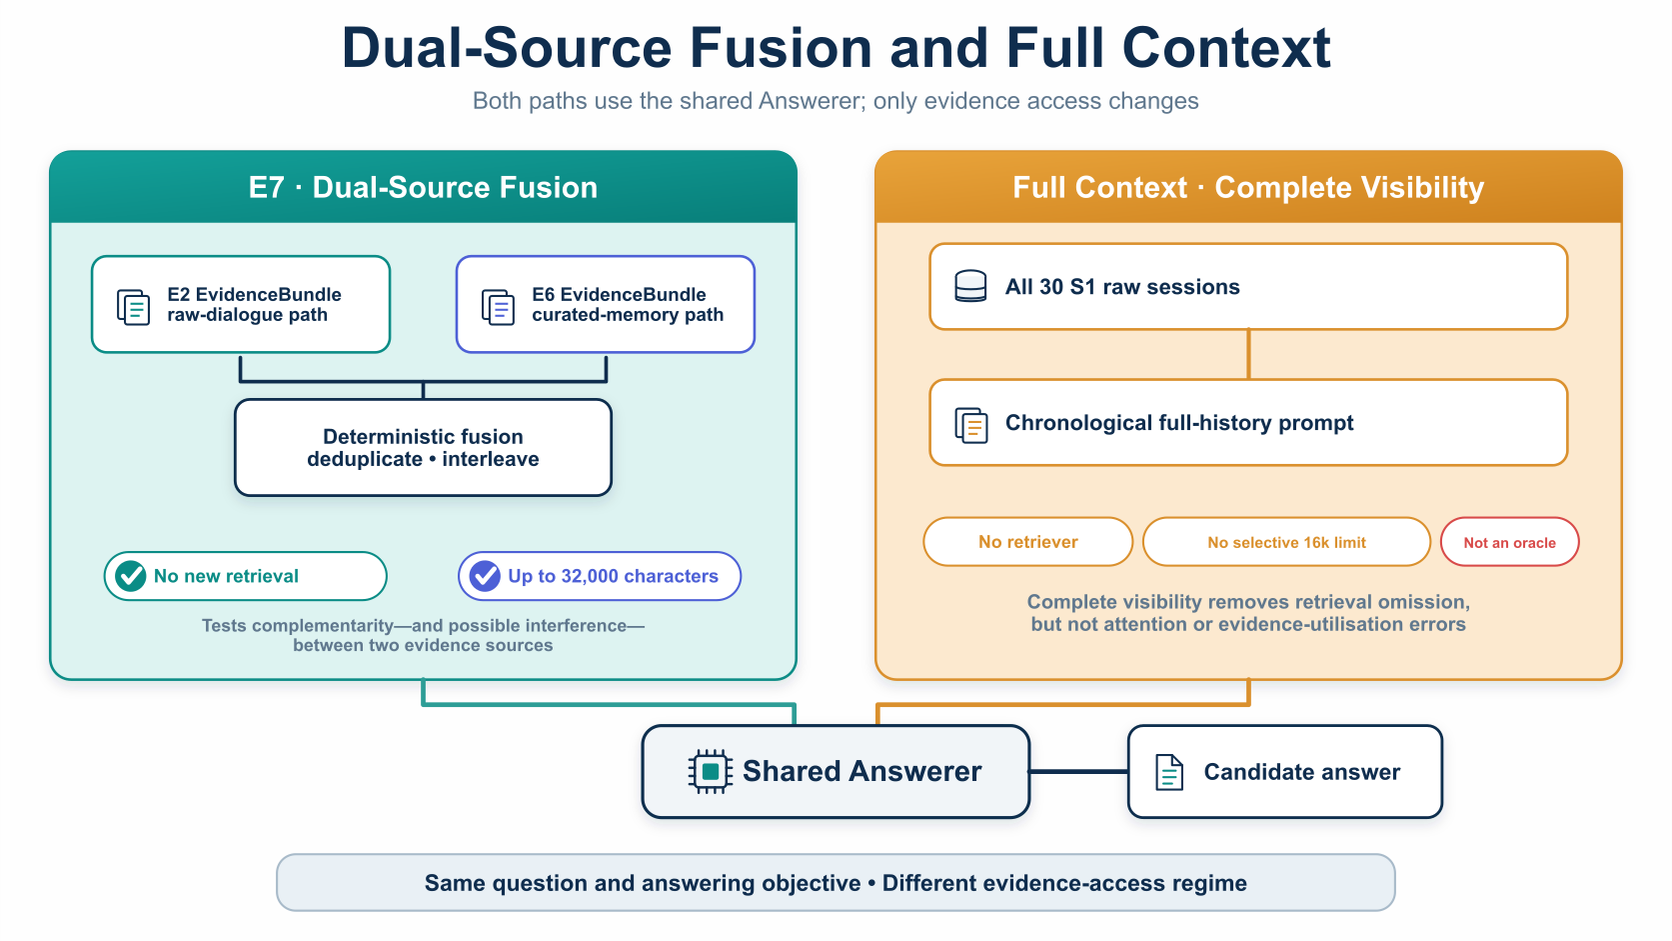
\includegraphics[width=0.68\linewidth,height=0.27\textheight,keepaspectratio]{../figures/chapter-3/figure-3-5-e7-fusion-vs-full-context.png}
  \caption{Comparison of E7 dual-source fusion and the Full Context diagnostic path. E7 deterministically combines the completed E2 and E6 EvidenceBundles without new retrieval, whereas Full Context exposes the complete ordered raw history without the selective 16,000-character limit. Both paths use the shared Answerer.}
  \label{fig:ch3-6}
\end{figure}

This chapter has defined the complete system graph. E1--E4 form the controlled raw-memory core, E5--E6 extend the design to agent-curated memory, E7 combines two completed evidence sources, and Full Context removes explicit retrieval as a diagnostic comparison. All selective conditions converge on the same EvidenceBundle and Answerer boundary.

Chapter~\ref{chap:ch4} instantiates this architecture as a controlled experiment. It consolidates the method constants defined here and specifies the frozen question set, backbone models, remaining run controls, execution protocol, evaluation metrics, and paired statistical analysis.
